\documentclass[12pt,fleqn]{article}
\usepackage{
    amsfonts,
    amsmath,
    amssymb,
    amsthm,
    booktabs,
    enumerate,
    flexisym,
    graphicx,
    setspace,
    slantsc,
    tabularx,
    url,
}

\date{2015-03-27}

\author{Gray Calhoun\thanks{Economics Department; Iowa State
    University; Ames, IA 50011. Telephone: (515) 294-6271.  Email:
    \guillemotleft gcalhoun@iastate.edu\guillemotright, web:
    \guillemotleft http://www.econ.iastate.edu/\textasciitilde
    gcalhoun\guillemotright.} \\
  Iowa State University}


\title{Graphing better Impulse Response Functions for discrete-time
  linear models}
% The LaTeX macros in this file are available through the CC0 license
% (creative commons public domain.  See
% <http://creativecommons.org/publicdomain/zero/1.0> for more
% details.)  To the extent possible under law, the copyright holders
% have waived all copyright and related or neighboring rights to the
% contents of this file.

\usepackage[letterspace=35]{microtype}
\newcommand{\allcaps}[1]{\textls{\MakeUppercase{#1}}}

\newcommand{\AIC}{\allcaps{AIC}}
\newcommand{\BIC}{\allcaps{BIC}}
\newcommand{\BRC}{\allcaps{BRC}}
\newcommand{\CDF}{\allcaps{CDF}}
\newcommand{\CLT}{\allcaps{CLT}}
\newcommand{\DGP}{\allcaps{DGP}}
\newcommand{\FCLT}{\allcaps{FCLT}}
\newcommand{\FWE}{\allcaps{FWE}}
\newcommand{\GDP}{\allcaps{GDP}}
\newcommand{\HAC}{\allcaps{HAC}}
\newcommand{\IRF}{\allcaps{IRF}}
\newcommand{\IRFs}{\allcaps{IRF}s}
\newcommand{\LLN}{\allcaps{LLN}}
\newcommand{\LM}{\allcaps{LM}}
\newcommand{\MA}{\allcaps{MA}}
\newcommand{\MDS}{\allcaps{MDS}}
\newcommand{\MSE}{\allcaps{MSE}}
\newcommand{\NBER}{\allcaps{NBER}}
\newcommand{\NSF}{\allcaps{NSF}}
\newcommand{\NED}{\allcaps{NED}}
\newcommand{\OLS}{\allcaps{OLS}}
\newcommand{\OOS}{\allcaps{OOS}}
\newcommand{\SFWE}{\allcaps{SFWE}}
\newcommand{\SPA}{\allcaps{SPA}}
\newcommand{\VAR}{\allcaps{VAR}}
\newcommand{\WFWE}{\allcaps{WFWE}}


\urlstyle{same}
\newcolumntype{C}{>{\centering\arraybackslash}X}

\usepackage[small]{caption}
\usepackage[T1]{fontenc}
\usepackage[margin=1.25in]{geometry}
\usepackage[charter]{mathdesign}
\usepackage[letterspace=35]{microtype}
\usepackage[sort,round,comma]{natbib}
\bibliographystyle{abbrvnat}
\newcommand\citepos[2][]{\citeauthor{#2}'s \citeyearpar[#1]{#2}}
\newcommand\poscw{\citeauthor{ClW:06}'s \citeyearpar{ClW:06,ClW:07}}
\newcommand\citen[1]{\citeauthor{#1}, \citeyear{#1}}

\renewcommand{\Re}{\operatorname{Re}}
\renewcommand{\Im}{\operatorname{Im}}

\DeclareMathOperator{\whitenoise}{\mathit{white\ noise}}
\DeclareMathOperator{\E}{E}
\DeclareMathOperator{\floor}{floor}
\DeclareMathOperator{\ceil}{ceil}
\newcommand{\vep}{\varepsilon}
\newcommand{\AR}{\allcaps{AR}}
\newcommand{\RR}{\mathbb{R}}
\newcommand{\VECM}{\allcaps{VECM}}

\newtheorem{prop}{Proposition}

\begin{document}
\maketitle
\begin{abstract}\noindent%
  We show how to construct continuous and differentiable
  Impulse Response Functions and for discrete-time \VAR s and Vector
  Error-Correction Models. Current methods produce piecewise linear
  functions that introduce visual distortions, especially when many
  response functions are plotted in the same graph to represent
  uncertainty or partial identification. We also show how to plot the
  cumulative response to a shock. In addition to being more accurate
  than current methods, our proposed approach is also much prettier.
\end{abstract}

\section{Introduction}

Impulse Response Functions (\IRF s) are widely used in Macroeconomics
to represent the dynamic effect over time of an unanticipated shock to
an economic system. Formally, if $\{y_t\}$ is a stationary sequence of
random vectors in $\RR^k$ and
\[
\E(y_{t+s} \mid y_t, y_{t-1},\dots) = g_s(y_t,\dots,y_{t-p})
\]
for each $s > 0$,%
\footnote{For later convenience, define
  $g_0(y_t,\dots,y_{t-p}) = y_t$ and $g_s = 0$ for $s < 0$.} %
the \IRF\ corresponding to the shock $\Delta$ is the difference
\[
\Psi_s(\Delta) = g_s(y_t + \Delta, y_{t-1},\dots,y_{t-p}) - g_s(y_t, y_{t-1},\dots,y_{t-p})
\]
viewed as a function of $s$.%
\footnote{Note that $\Psi_0(\Delta) = \Delta$ and $\Psi_s(\Delta) = 0$ for $s <
  0$.} %
Obviously the values of the \IRF\ depend on the specific nature of the
shock $\Delta$, and different choices of $\Delta$ can correspond to
different shocks of theoretical interest.  In Macroeconomic
applications, $t$ and $s$ are typically integers and $g_s$ is often
derived from a recursive linear model, the \VAR
\begin{equation}\label{eq:1}
  y_t = A_0 + A_1 y_{t-1} + \cdots + A_p y_{t-p} + \vep_t
\end{equation}
where $\vep_t$ is a martingale difference sequence is one example.

It is straightforward to calculate the values of the \IRF s for
integer-values of $s$ in models like~\eqref{eq:1}.
Note that
\begin{align*}
  g_1(y_t,\dots,y_{t-p}) &= \E(y_{t+1} \mid y_t, y_{t-1},\dots) \\
  &= A_0 + A_1 y_{t} + \cdots + A_p y_{t-p+1}
\end{align*}
and
\begin{align*}
  g_s(y_t,\dots,y_{t-p})
  &= \E(y_{t+s} \mid y_t, y_{t-1},\dots) \\
  &= \E( \E(y_{t+s} \mid y_{t+s-1}, y_{t+s-2},\dots) \mid y_t, y_{t-1},\dots) \\
  &= \E( A_0 + A_1 y_{t+s-1} + \cdots + A_p y_{t+s-p} \mid y_t, y_{t-1},\dots) \\
  &= A_0 + A_1 \E(y_{t+s-1} \mid y_t, y_{t-1},\dots) + \cdots + A_p \E(y_{t+s-p} \mid y_t, y_{t-1},\dots) \\
  &= A_0 + A_1 g_{s-1}(y_t,\dots,y_{t-p}) + \cdots + A_p g_{s-p}(y_t,\dots,y_{t-p})
\end{align*}
for $s > 1$, which can be calculated recursively for $s =
2,3,\dots$. Then
\begin{equation*}
  \Psi_1(\Delta) = A_1 \Delta
\end{equation*}
and, for $s > 1$,
\begin{align*}
  \Psi_s(\Delta)
  &= g_s(y_t + \Delta,\dots,y_{t-p}) - g_s(y_t,\dots,y_{t-p}) \\
  &= \sum_{\ell = 1}^{p} A_\ell \big[g_{s-\ell}(y_t+\Delta,\dots,y_{t-p}) - g_{s-\ell}(y_t,\dots,y_{t-p})\big] \\
  &= \sum_{\ell = 1}^{p} A_\ell \Psi_{s-\ell}(\Delta)
\end{align*}
which can again be calculated recursively. In some applications this
is enough. But in most applications, it is necessary to graph the \IRF
s and to connect the points; this is especially important when more
than one \IRF\ is plotted on the same graph --- whether to represent
dynamics under different assumptions (see \citealp{BeM:98}, and
\citealp{StW:01}, for representative examples), to represent
statistical uncertainty (\citealp{Kil:98}, and \citealp{SiZ:99}) or to
represent regions that are partially identified (\citealp{Uhl:05}, and
\citealp{InK:13}). So far, representing these dynamics has been
achieved by linear interpolation, so
\begin{equation*}
  \Psi_s(\Delta) = (s - \floor(s)) \, \Psi_{\ceil(s)}(\Delta) + (\ceil(s) - s) \, \Psi_{\floor(s)}(\Delta)
\end{equation*}
for noninteger $s$, where $\floor(s)$ and $\ceil(s)$ represent the
largest integer less than $s$ and smallest integer value greater than
$s$ respectively. Unfortunately, this method introduces misleading
visual distortions, which we will explicitly discuss later.

In this paper, we show how the \IRF\ $\Psi_s(\Delta)$ can be meaningfully
defined for \VAR s for any real positive value of $s$ and give a
convenient method for calculating it. (Figures~\ref{f1} and~\ref{f2}
have examples if you're impatient to see them.) This allows
researchers to use the \VAR\ itself to interpolate between the points
for which it is usually defined and results in graphs that do not have
the distortions produced by linear interpolation. In the next section,
we offer a simple example of our approach that motivates the general
technique. Sections~\ref{recommended} and~\ref{extensions} explain the
methods in general and provide some extensions to cumulative responses
and Vector Error Correction Models, and Section~\ref{example} provides
a numerical example.

\section{Motivation}

\begin{figure}[t]
  \centering
  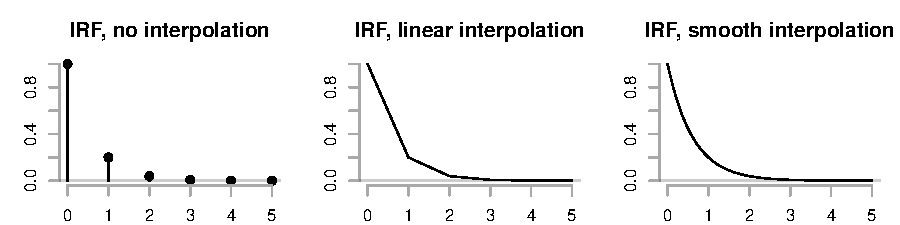
\includegraphics{graphs/motivation.pdf}
  \caption{\IRF\ for simple AR(1) example. Here $y_t = 0.2 y_{t-1} +
    \vep_t$ --- the vertical axis shows $\Psi_x(1)$. The left panel
    plots only integer values of $x$, the middle panel uses linear
    interpolation between the integers, and the right panel plots the
    function $0.2^x$ directly.}
  \label{f0}
\end{figure}

For motivation, start with the simplest univariate case and assume
that $y_t$ is the \AR(1)
\begin{equation*}
y_t = a y_{t-1} + \vep_t
\end{equation*}
It is well-known that the recursive definitions used in the first
section imply that $\Psi_s(\Delta) = a^s \Delta$.  When $a > 0$, this
function is well-defined for all positive real $s$, and can be used
directly to interpolate between the integer points. Figure~\ref{f0}
plots $\Psi_s(\Delta)$ for $\Delta = 1$ and $a = 0.2$ using three
approaches: first only for the integer values of $s$, second using
linear interpolation between the integer values, and finally using
$a^s \Delta$ directly for all $s \geq 0$.%
\footnote{All of the graphs in this paper were produced using
  \citet{R}} %
While one could debate which of the functions represents the ``true''
impact at a fractional point in time, the right panel --- using
$0.2^s$ directly --- more clearly expresses the shock's rate of decay
and, equivalently, the dynamics of the \AR\ model.

This clarity should not be surprising. We can see that $\Psi_s(\Delta)
= a^s \Delta$ satisfies the recurrence relation implied by the lag
structure of the original \AR\ process for any positive real value of
$s$:
\begin{equation*}
  \Psi_s(\Delta) = a^s \Delta = a \times a^{s-1} \Delta = a \, \Psi_{s-1}(\Delta).
\end{equation*}
For the methods we propose in this paper we will see that this
condition holds in general: if $\Phi(L)$ is the lag polynomial of the
\VAR (so $\Phi(L)y_t = \vep_t$ for $t = 1, 2, \dots$), then $\Phi(L)
\Psi_s(\Delta) = 0$ for all $s \in \RR^+$.%
\footnote{We have implicitly defined $L \Psi_s(\Delta) =
  \Psi_{s-1}(\Delta)$.} %
This condition only holds for integer values of $s$ when
$\Psi_s(\Delta)$ is constructed by linear interpolation.

\begin{figure}[t]
  \centering
  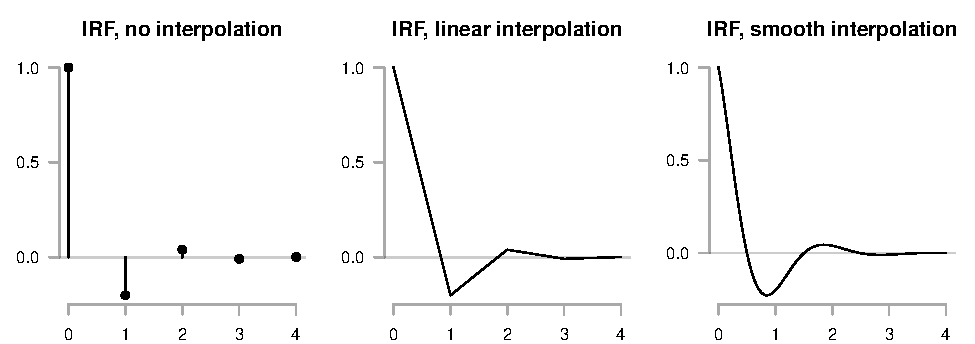
\includegraphics{graphs/motivation2.pdf}
  \caption{\IRF\ for simple AR(1) example. Here $y_t = -0.2 y_{t-1} +
    \vep_t$ --- the vertical axis shows $\Psi_x(1)$. The left panel
    plots only integer values of $x$, the middle panel uses linear
    interpolation between the integers, and the right panel plots the
    function $|a|^x \cos(\pi x)$ directly.}
  \label{f0b}
\end{figure}

The case $a \in (-1, 0)$ is slightly more complicated.  The
previous solution, $a^s \Delta$, continues to be well-defined and has a real value
for all integer values of $s$, but is not for non-integer
values. However, for any integer value of $s$ the equality
\begin{equation*}
  a^s = |a|^s \cos(\pi s)
\end{equation*}
holds, so $\Psi_s(\Delta) = |a|^s \cos(\pi s) \Delta$ agrees with $a^s
\Delta$ on integer values and is well-defined and real-valued for
non-integer values. Moreover, this choice of $\Psi_s(\Delta)$
satisfies the recurrence relation for the \AR(1) model (when $a < 0$)
just as before:
\begin{equation*}
  \Psi_s(\Delta) = |a|^s \cos(\pi s) \cdot \Delta = - |a| \times |a|^{s-1} \cos(\pi (s-1)) \cdot \Delta = a \, \Psi_{s-1}(\Delta)
\end{equation*}
implying
\begin{equation*}
  (1 - a L) \, \Psi_s(\Delta) = 0.
\end{equation*}
Since it is exactly correct on the integers and satisfies the model's
dynamics for noninteger values as well, this choice of $\Psi$ is a
sensible choice for interpolating between the
integers. Figure~\ref{f0b} plots the \IRF s for $a = -0.2$ and $\Delta
= 1$ with no interpolation, linear interpolation, and our definition
of $\Psi_s(\Delta)$. The smooth version more accurately reflects the
system's dynamics again.

This choice of $\Psi_s(\Delta)$ was not made at random. Any complex
number $a + bi$ can be written in polar form,
\[
a + bi = R [\cos(\theta) - i \sin(\theta)]
\]
where $R = |a^2 + b^2|^{1/2}$ and $\theta$ satisfies $\cos(\theta) = a/R$ and
$\sin(\theta) = b/R$; then real powers can be defined easily as%
\footnote{See \citet{Ham:94} for an introduction.} %
\[
(a + bi)^s = R^s [\cos(\theta s) - i \sin(\theta s)].
\]
For the \AR\ example above, $a < 0$ and $b = 1$ implies that $\theta =
\pi$, giving $a^s = |a|^s \cos(\pi s)$ as we originally claimed. This
example also suggests a more general method: for any \VAR\ we can
solve the recurrence relation using standard tools (as described in
\citealp{Ham:94}, for example) and use that solution as the \IRF\ for
real-valued $s$. We pursue that approach in the next section.

\section{General Approach}\label{recommended}

The \AR(1) model in the previous section can be extended to general
\VAR s using the ``canonical'' representation.%
\footnote{See Chapter 1 of \citet{Ham:94} for a textbook treatment of
  much of this material.} %
Define $y_t$ as in Equation~(\ref{eq:1}), so
\[
y_t = \sum_{j=1}^p A_j y_{t-j} + \vep_t.
\]
To represent this relationship as a \VAR(1), form the vector
$(y_t',\dots,y_{t-p+1}')'$ and observe that
\[
\underbrace{\begin{pmatrix}
  y_t \\ y_{t-1} \\ y_{t-2} \\ \vdots \\ y_{t-p+1}
\end{pmatrix}}_{Z_t}
=
\underbrace{\begin{pmatrix}
  A_1 & A_2 & \cdots & A_{p-1} & A_p \\
  I_k & 0   & \cdots & 0 & 0 \\
  0  & I_k  & \cdots & 0 & 0 \\
  \vdots & \vdots & \ddots & \vdots & \vdots \\
  0 & 0 & \cdots & I_k & 0
\end{pmatrix}}_{F}
\underbrace{\begin{pmatrix}
  y_{t-1} \\ y_{t-2} \\ y_{t-3} \\ \vdots \\ y_{t-p}
\end{pmatrix}}_{Z_{t-1}}
+
\underbrace{\begin{pmatrix}
  \vep_{t} \\ 0 \\ 0 \\ \vdots \\ 0
\end{pmatrix}}_{U_t}.
\]n
So this relationship is equivalent to $Z_t = F Z_{t-1} + U_t$.

If the matrix $F$ has $q$ distinct
eigenvalues, it can be decomposed as
\[
F = M J M^{-1}
\]
where $J$ is block diagonal of the form
\[
J = \begin{pmatrix}
  J_1 & \cdots & 0 \\
  \vdots & \ddots & \vdots \\
  0 & \cdots & J_q
\end{pmatrix}
\]
and each $J_\ell$ is $m_\ell \times m_\ell$ of the form
\[
J_\ell =
\begin{pmatrix}
  \lambda_\ell & 1 & 0 & \cdots & 0 & 0 \\
  0 & \lambda_\ell & 1 & \cdots & 0 & 0 \\
  0 & 0 & \lambda_\ell & \cdots & 0 & 0 \\
  \vdots & \vdots & \vdots & \ddots & \vdots & \vdots \\
  0 & 0 & 0 & \cdots & \lambda_\ell & 1 \\
  0 & 0 & 0 & \cdots & 0 & \lambda_\ell
\end{pmatrix}
\]
where $\lambda_1,\dots,\lambda_q$ are the distinct eigenvalues of $F$
and $m_\ell$ is the number of times the $\ell$th eigenvalue is
repeated.  If all of the eigenvalues of $F$ are distinct, this is just
the eigenvalue decomposition of $F$.

This representation is convenient because, for positive integer values
of $s$, we have
\[
F^s = M J^s M^{-1}
\]
and
\begin{align*}
J^s           & =
\begin{pmatrix}
  J_1^s                  & \cdots                 & 0                                                                        \\
  \vdots                 & \ddots                 & \vdots                                                                   \\
  0                      & \cdots                 & J_q^s
\end{pmatrix},
\intertext{where}
J_\ell^s         & =
\begin{pmatrix}
  \lambda_\ell^s & \binom{s}{1} \lambda_\ell^{s-1} & \binom{s}{2} \lambda_\ell^{s-2} & \cdots & \binom{s}{m_\ell} \lambda_\ell^{s-m_\ell}     \\
  0           & \lambda_\ell^s            & \binom{s}{1} \lambda_\ell^{s-1} & \cdots & \binom{s}{m_\ell-1} \lambda_\ell^{s-m_\ell+1} \\
  0           & 0                      & \lambda_\ell^s            & \cdots & \binom{s}{m_\ell-2} \lambda_\ell^{s-m_\ell+2} \\
  \vdots      & \vdots                 & \vdots                 & \cdots & \vdots                         \\
  0           & 0                      & 0                      & \cdots & \lambda_\ell^s \\
\end{pmatrix} \\
&=
\begin{pmatrix}
  h_\ell(s,0) & h_\ell(s,1) & h_\ell(s,2) & \cdots & h_\ell(s,m_\ell)   \\
  0        & h_\ell(s,0) & h_\ell(s,1) & \cdots & h_\ell(s,m_\ell-1) \\
  0        & 0        & h_\ell(s,0) & \cdots & h_\ell(s,m_\ell-2) \\
  \vdots   & \vdots   & \vdots   & \ddots & \vdots      \\
  0        & 0        & 0        & \cdots & h_\ell(s,0)    \\
\end{pmatrix} \\
\intertext{and}
h_\ell(s,j) &=
\begin{cases}
  |\lambda_\ell|^s \big[\cos(\theta_\ell s) + i \sin(\theta_\ell s)\big] & j = 0 \\
  \frac{s!}{j!(s-j)!} |\lambda_\ell|^s \big[\cos(\theta_\ell s) + i \sin(\theta_\ell s)\big] & \text{if } s \geq j > 0 \\
  0 & \text{otherwise.}
\end{cases}
\end{align*}
where $\cos(\theta_\ell) = \Re(\lambda_\ell)/|\lambda_\ell|$ and
$\sin(\theta_\ell) = \Im(\lambda_\ell)/|\lambda_\ell|$ as above.

Then we can write
\begin{multline}\label{eq:6}
  F^s =
  \sum_{j = 1}^q \sum_{l=0}^{\min(m_\ell, \floor(s))} \tfrac{s(s-1)\cdots(s-l+1)}{l (l - 1) \cdots 1} |\lambda_j|^{s-l} \\
  \times\Big\{\big[A_{jl} \cos(\theta_j s) + B_{jl} \sin(\theta_j s)\big] + i\big[C_{jl} \cos(\theta_j s) + D_{jl} \sin(\theta_j s)\big]\Big\}
\end{multline}
where the coefficient matrices $A_{jl}$, $B_{jl}$, $C_{jl}$, and
$D_{jl}$ are chosen to match $F^0, F^1, F^2,\dots$.
For integer values of $s$, the imaginary components of $M J^s M^{-1}$
exactly cancel, so
\begin{equation*}
  0 = \sum_{j = 1}^q \sum_{l=0}^{\min(m_\ell, \floor(s))} \tfrac{s(s-1)\cdots(s-l+1)}{l (l - 1) \cdots 1} |\lambda_j|^{s-l}
  \big[C_{jl} \cos(\theta_j s) + D_{jl} \sin(\theta_j s)\big]
\end{equation*}
and we can use the real part alone, giving
\begin{equation}\label{eq:7}
  F^s =
  \sum_{j = 1}^q \sum_{l=0}^{\min(m_\ell, \floor(s))} \tfrac{s(s-1)\cdots(s-l+1)}{l (l - 1) \cdots 1} |\lambda_j|^{s-l} \big[A_{jl} \cos(\theta_j s) + B_{jl} \sin(\theta_j s)\big]
\end{equation}
to produce $F^1, F^2, F^3,\dots$. Our proposal, in a nutshell, is to
use the definition given by \eqref{eq:7} for all of the reals rather
than just the integers, exactly as we did in the motivating \AR(1)
examples.

Equation~\eqref{eq:6} has another practical implication. Although
$F^s$ has real and imaginary components for real $s$, we are only
interested in its real component, which generates the \IRF s for
integer values of $s$. So rather than working out the matrices
$A_{jl}$ and $B_{jl}$ to use~\eqref{eq:7}, we can calculate the
complex valued $F^s$ and simply drop its imaginary component. This
calculation is directly available in many programming languages and
can be implemented as $M J^s M^{-1}$ using the Jordan decomposition if
it is not.

We conclude this section with a formal statement of the result.

\begin{prop}[Impulse Response Functions for \VAR s]\label{prop1}
  Let $F$ be the coefficient matrix of the canonical \VAR(1)
  representation of an arbitrary \VAR($p$), and let $M$ and $J$ be the
  matrices of its Jordan decomposition, so $F = M J
  M^{-1}$. Define $\Psi_s(\Delta)$ as the first $k$ elements of the
  vector $\Re(M J^s M^{-1}) \Delta_0$ for all $s \in [0,+\infty)$, where
  $\Delta_0 = (\Delta', 0')'$.

  Then
  \begin{equation*}
    \Psi_s(\Delta) = \sum_{j=1}^q A_j \Psi_{s-j}(\Delta)
  \end{equation*}
  for all $s > 0$, so $\Psi_s(\Delta)$ satisfies the recurrence
  relation implied by the original \VAR.
\end{prop}
\begin{proof}
  Observe that the series $a_s = \Re(F^s) \Delta_0$ satisfies
  $a_s = F a_{s-1}$, since $F$ is real and
  \[
    F a_{s-1} = F \Re(F^{s-1}) \Delta_0
    = \Re(F^s) \Delta_0
    = a_s.
  \]
  The conclusion of this proposition is a direct consequence.
\end{proof}

\section{Cumulative response and other extensions}\label{extensions}

The results in the previous section will work for many applications,
but in others we may may be interested in other functions of the
variables. An example is if $y_t$ represents differenced variables,
(say, the first difference of log GDP), but we are interested in the
response on the level of the variable. A different but very similar
issue arises if the model of interest is a Vector Error Correction
Model (\VECM) model and not a \VAR. In these cases, we can augment the
canonical form used earlier to derive a new \VAR(1) representation,
and then apply our earlier techniques. We'll demonstrate this approach
for these two examples.

First, suppose that $y_t$ has a stationary \VAR($p$) representation as
before, but now we want to derive the response on some elements of the
vector $S_t = \sum_{s=0}^t y_s$. Immediately we have $S_t - y_t =
S_{t-1}$, so we can extend the canonical representation for $y_t$ by
adding $S_t$ as the first element of the vector $Z_t$. Observe that
\begin{equation*}
  \begin{pmatrix}
    S_t - y_t \\ y_t \\ y_{t-1} \\ y_{t-2} \\ \vdots \\ y_{t-p+1}
  \end{pmatrix}
  =
  \begin{pmatrix}
    I & 0 & 0 & \cdots & 0 & 0 \\
    0 & A_1 & A_2 & \cdots & A_{p-1} & A_p \\
    0 & I   & 0 & \cdots & 0 & 0 \\
    0 & 0   & I & \cdots & 0 & 0 \\
    \vdots & \vdots & \vdots & \ddots & \vdots & \vdots \\
    0 & 0 & 0 & \cdots & I & 0
  \end{pmatrix}
  \begin{pmatrix}
    S_{t-1}  \\ y_{t-1} \\ y_{t-2} \\ \vdots \\ y_{t-p+1} \\ y_{t-p}
  \end{pmatrix}
  +
  \begin{pmatrix}
    0 \\ \vep_t \\ 0 \\ 0 \\ \vdots \\ 0
  \end{pmatrix}.
\end{equation*}
And this equation can be rewritten as
\begin{equation*}
  \begin{pmatrix}
    S_t \\ y_t \\ y_{t-1} \\ y_{t-2} \\ \vdots \\ y_{t-p+1}
  \end{pmatrix}
  =
  \begin{pmatrix}
    I & A_1 & A_2 & \cdots & A_{p-1} & A_p \\
    0 & A_1 & A_2 & \cdots & A_{p-1} & A_p \\
    0 & I   & 0 & \cdots & 0 & 0 \\
    0 & 0   & I & \cdots & 0 & 0 \\
    \vdots & \vdots & \vdots & \ddots & \vdots & \vdots \\
    0 & 0 & 0 & \cdots & I & 0
  \end{pmatrix}
  \begin{pmatrix}
    S_{t-1}  \\ y_{t-1} \\ y_{t-2} \\ \vdots \\ y_{t-p+1} \\ y_{t-p}
  \end{pmatrix}
  +
  \begin{pmatrix}
    \vep_t \\ \vep_t \\ 0 \\ 0 \\ \vdots \\ 0
  \end{pmatrix}.
\end{equation*}
This representation is now a \VAR(1) that can be handled exactly as above.

The \VECM\ model is similar. Suppose now that we have the stationary
relationship
\begin{equation*}
  \Delta y_t = B y_{t-1} + A_1 \Delta y_{t-1} + \cdots + A_p \Delta
  y_{t-p} + \vep_t.
\end{equation*}
This can also be put in a canonical form using almost identical
arguments as before
\begin{equation*}
  \begin{pmatrix}
    y_t \\ \Delta y_t \\ \Delta y_{t-1} \\ \Delta y_{t-2} \\ \vdots \\
    \Delta y_{t-p+1}
  \end{pmatrix}
  =
  \begin{pmatrix}
    (I + B) & A_1 & A_2 & \cdots & A_{p-1} & A_p \\
    B & A_1 & A_2 & \cdots & A_{p-1} & A_p \\
    0 & I   & 0   & \cdots & 0 & 0 \\
    0 & 0   & I   & \cdots & 0 & 0 \\
    \vdots & \vdots & \vdots & \ddots & \vdots & \vdots \\
    0 & 0 & 0 & \cdots & I & 0
  \end{pmatrix}
  \begin{pmatrix}
    y_{t-1} \\ \Delta y_{t-1} \\ \Delta y_{t-2} \\ \vdots \\ \Delta y_{t-p+1} \\
    \Delta y_{t-p}
  \end{pmatrix}
  +
  \begin{pmatrix}
    \vep_t \\ \vep_t \\ 0 \\ 0 \\ \vdots \\ 0
  \end{pmatrix}
\end{equation*}
In both cases, we can now define the \IRF\ using the canonical \VAR(1)
representation.

\section{Numerical example}\label{example}

For a numerical example, consider the two-variable \VAR(2)
\begin{equation}\label{eq:2}
  \begin{pmatrix}
    y_{1t} \\ y_{2t}
  \end{pmatrix}
  =
  \begin{pmatrix}
    - 0.5 & 0.01 \\ 0.3 & 0.1
  \end{pmatrix}
  \begin{pmatrix}
    y_{1,t-1} \\ y_{2,t-1}
  \end{pmatrix}
  +
  \begin{pmatrix}
    -0.2 & 0.1 \\ -0.1 & 0.0
  \end{pmatrix}
  \begin{pmatrix}
    y_{1,t-2} \\ y_{2,t-2}
  \end{pmatrix}
  +
  \begin{pmatrix}
    \vep_{1t} \\ \vep_{2t}
  \end{pmatrix}
\end{equation}
and assume for the sake of argument that $(\vep_{1t},\vep_{2t}) \sim
N(0,I)$ represents the shocks of interest.

As described above, we will define the smooth \IRF s for a shock to
the first element as
\begin{equation*}
  \begin{pmatrix}
    \hat y_{1s} \\ \hat y_{2s}
  \end{pmatrix}
  =
  \begin{pmatrix}
    1 & 0 & 0 & 0 \\ 0 & 1 & 0 & 0
  \end{pmatrix}
  M J^s M^{-1}
  \begin{pmatrix}
    1 \\ 0 \\ 0 \\ 0
  \end{pmatrix}
\end{equation*}
with $M$ and $J$ the Jordan decomposition of the matrix
\begin{equation}
F = \begin{pmatrix}
    - 0.5 & 0.01 & -0.2 & 0.1 \\
      0.3 & 0.1 & -0.1 & 0.0 \\
      1.0 & 0.0 & 0.0 & 0.0 \\
      0.0 & 1.0 & 0.0 & 0.0
  \end{pmatrix}
\end{equation}
The same equations hold for the \IRF s for a shock to the second
element of $y_t$, but now the last vector should be $(0, 1, 0, 0)'$.

\begin{figure}[t]
  \centering
  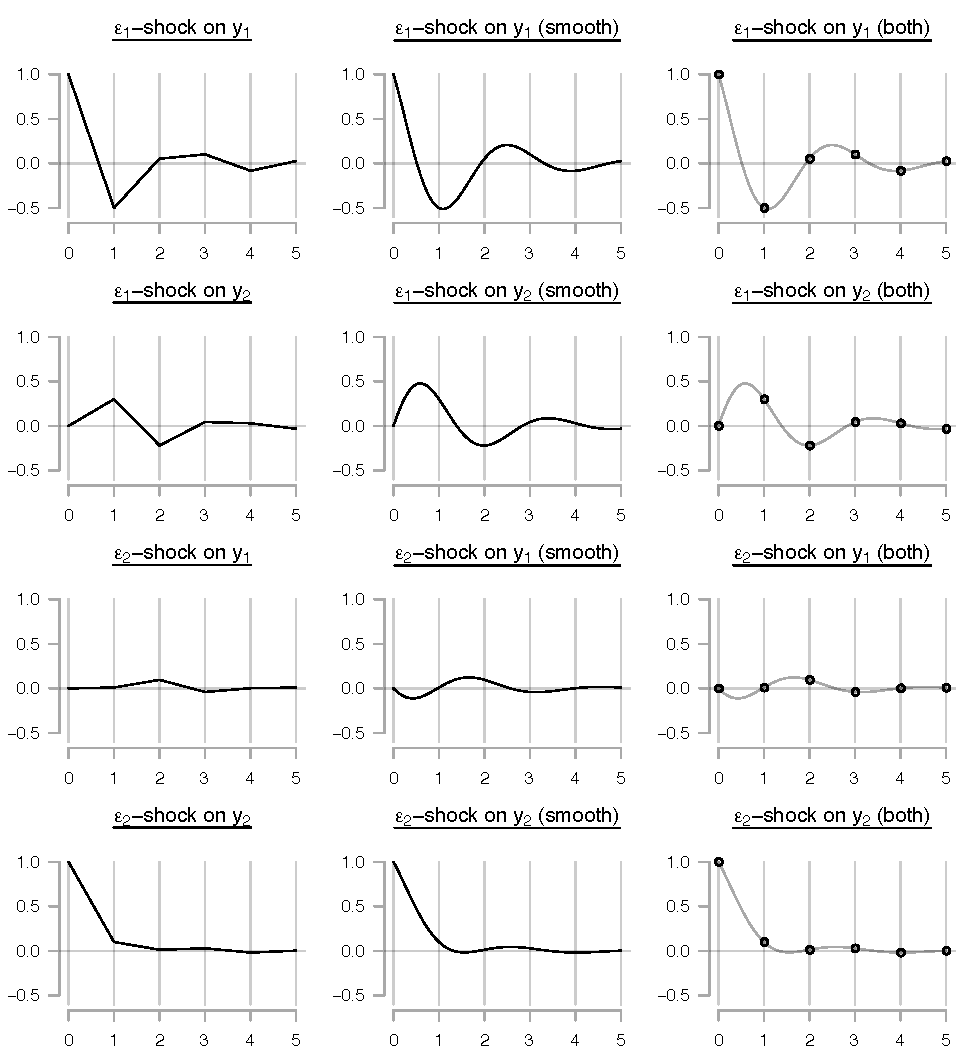
\includegraphics{graphs/numeric.pdf}
  \caption{Impulse Response Functions from Section~\ref{example}
    example; $y_t$ is generated by Equation~\eqref{eq:2}. The left
    column plots standard \IRF s and the right column plots our new
    method.}
  \label{f1}
\end{figure}

We plot the \IRF s in Figure~\ref{f1}. The first column plots the
standard \IRF s and the second plots our proposed smooth
plots. Although the general impressions from both graphs are similar,
there are important differences. First, peaks and troughs are often
underestimated by the standard \IRF s and their timing is frequently
misidentified. This is especially apparent in the first peak in the
second row. Second, even the sign of the \IRF\ can be misidentified,
as we see with the immediate response of $y_{1t}$ to a shock in
$y_{2t}$. Finally, unless turning points in the smooth functions
happen to coincide with integer values, discretizing the \IRF s
introduces misleading asymmetries and kinks.

\begin{figure}[t]
  \centering
  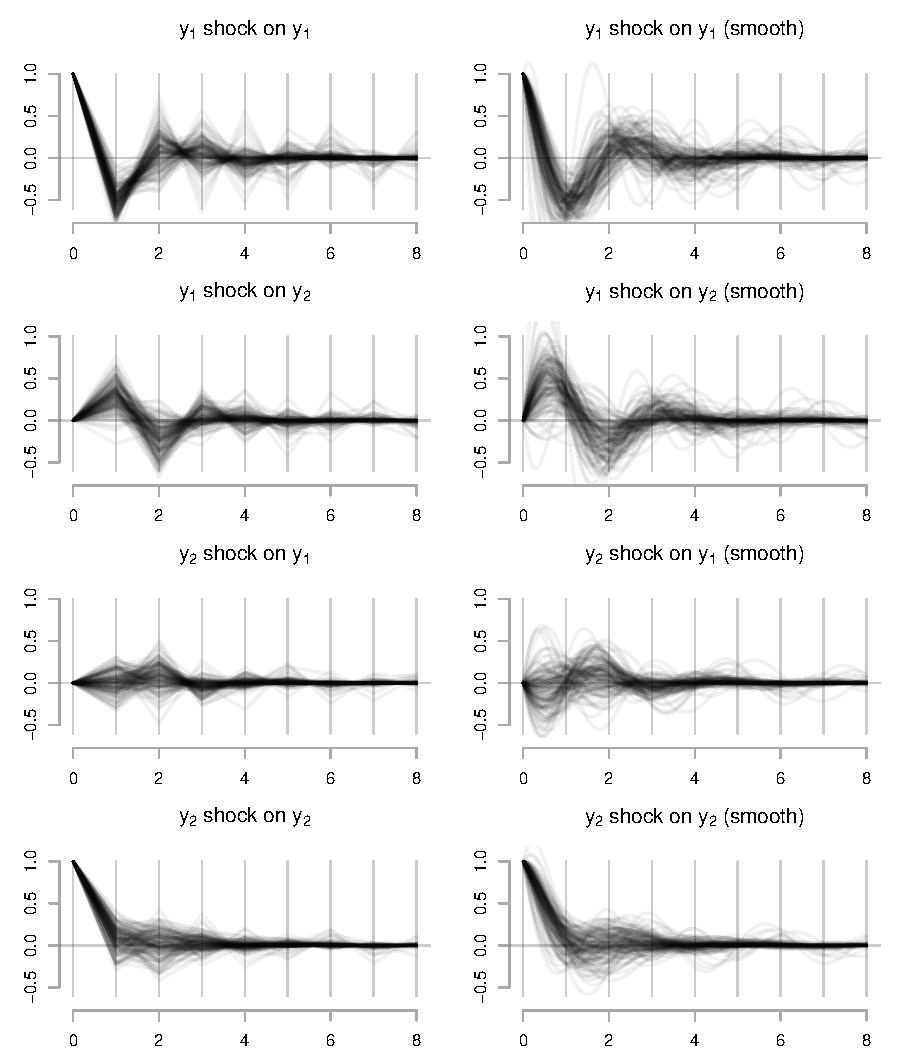
\includegraphics{graphs/numeric2.pdf}
  \caption{Impulse Response Functions from Section~\ref{example}
    example; $y_t$ is generated by Equation~\eqref{eq:2}, with
    independent $N(0,0.15)$ random variable added to each
    coefficient. These graphs plot the \IRF s from 150 independent
    draws of the coefficient matrices. The left column plots standard
    \IRF s and the right column plots our new method.}
  \label{f2}
\end{figure}

These distortions are even more apparent when we graph multiple
perturbations of the \IRF s in the same panel, which is a common way
of representing uncertainty or set-identified responses. To
demonstrate this phenomenon, we generated 150 replications of the \IRF
s by adding independent N(0, 0.15) noise terms to each element of $A$,
and then plotting the implied \IRF s as before.

These graphs are shown in Figure~\ref{f2}. The same issues apparent in
Figure~\ref{f1} are present here as well. But there are other problems
as well. In the first curve, for example, the discrete \IRF\ shows
that there is substantial negative correlation between the period 2
and period 3 estimated response and the period 3 and 4 response. But
the smoothed graph makes it clear that this is driven by the timing
and size of the first peak. When that peak is near period 2, the curve
has time to fall noticeably before period 2, but when the peak is
closer to period 3, the curve is still rising for that interval. The
actual dynamics implied by the different curves are very
similar. Similar but less dramatic distortions appear in the other
panels as well. In the third row, for example, the discrete \IRF\
shows that about half of the parameter values have an initial increase
in response to a $y_{20}$ shock and half have an initial decrease, but
the smooth curves show that virtually all of them have an immediate
decrease, but that many start to increase very soon. The exact
location of the peak that falls between periods 1 and 2 determines
most of the initial dynamics, but this is impossible to see in the
discrete curve.

\section{Discussion}

Vector Autoregressive models do not just have implications for the
period-to-period dynamics of a stochastic process, they also have
implications about the very short-run dynamics within periods. In this
paper, we propose that researchers graph those intra-period dynamics
when plotting \IRF s and we give a simple method to do so, based on
the \VAR's canonical \VAR(1) representation. Even when researchers do
not want to assign any economic importance to these ultra short-run
dynamics, plotting them in the \IRF s minimizes visual distortions
that can arise from discretizing the dynamics, especially when several
\IRF s are plotted over each other to represent uncertainty or set
identification --- see Figure~\ref{f2} for an example.

\bibliography{localrefs,latex_misc/references}
\end{document}
